\chapter*{Premessa}
\graphicspath{ {./images/primepagine/} }

di Marina Frua

“Memorie della De Angeli Frua che meritano di essere conosciute e trasmesse”

\begin{figure}[h]
	\centering
		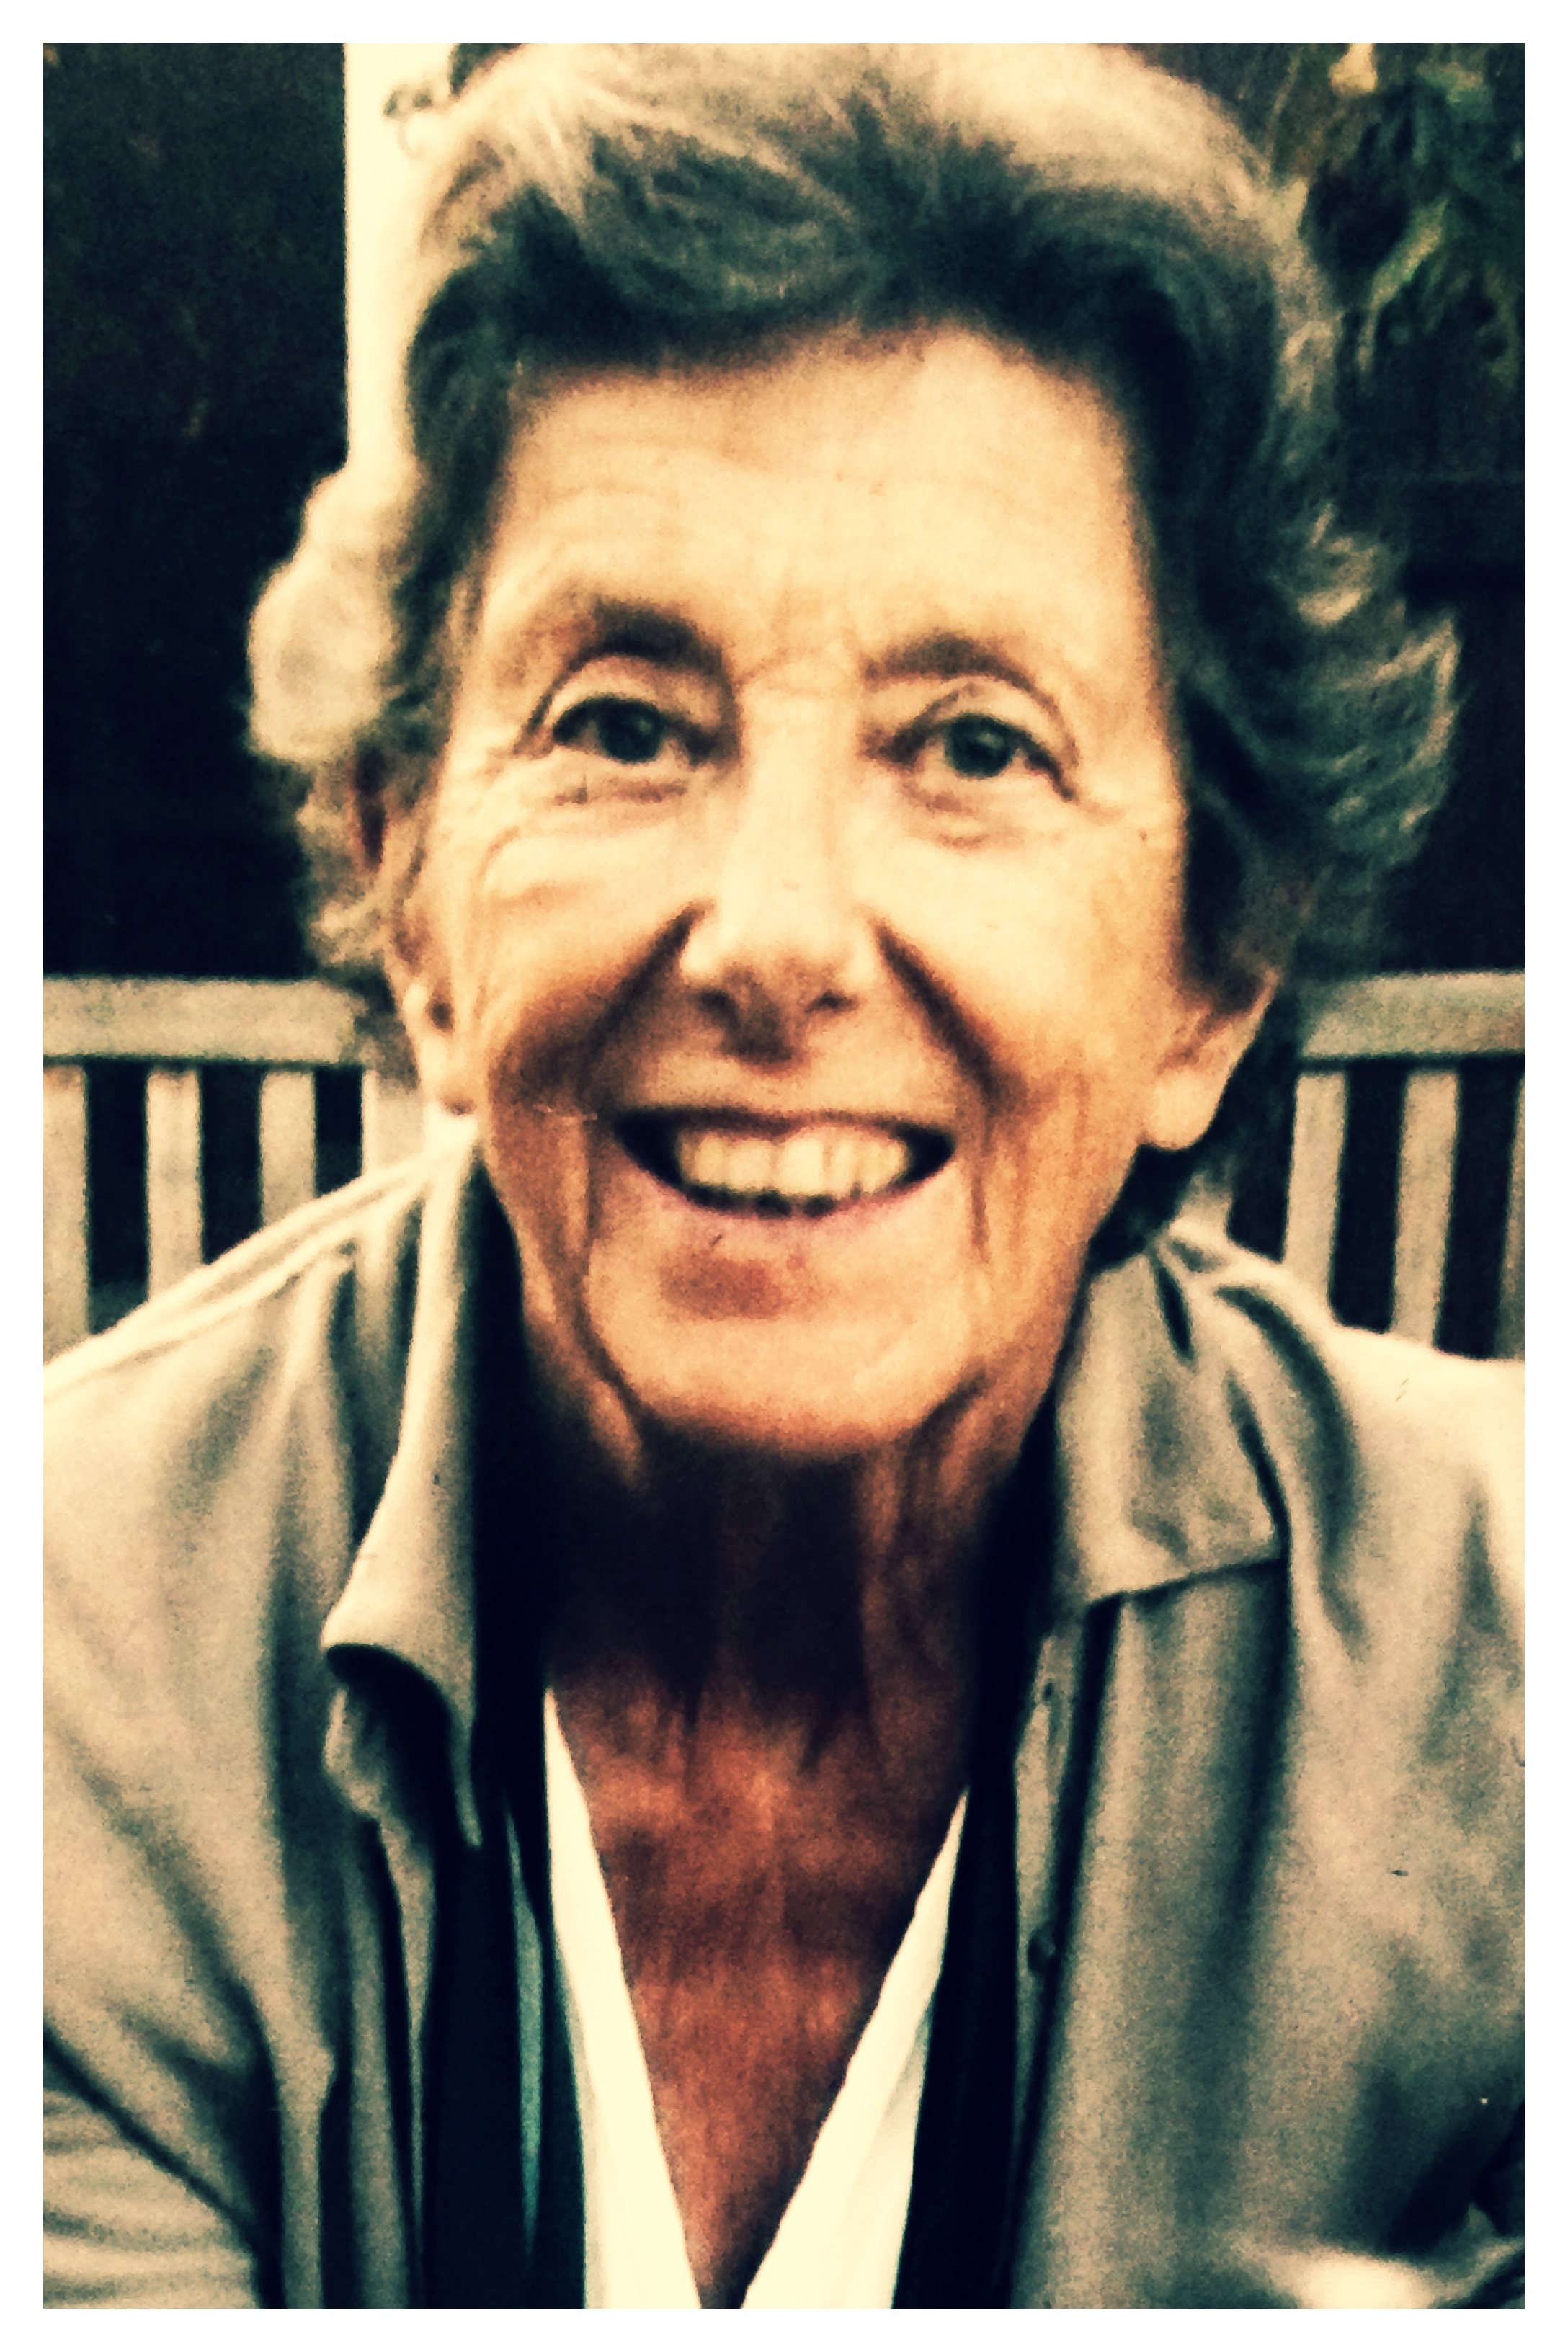
\includegraphics[width=\textwidth]{marina_frua.jpg}
	\caption{}
	\label{fig:marina_frua}
\end{figure}

A Milano in via Paleocapa al numero uno, una bella casa di quattro piani vicino alla Stazione Nord e al Parco Sempione, abitavano i De Angeli e i Frua.
   Ernesto De Angeli, senatore del Regno, e le sue belle, severe e impettite sorelle occupavano il primo e il secondo piano. Giuseppe Frua abitava al terzo piano e Alberto, figlio di Giuseppe, al quarto.
   Io facevo parte della famiglia di Alberto: ero piccola e di questi personaggi, all’epoca così importanti, ho un ricordo forse un po’ sbiadito ma a tratti intenso. 
   Sovente andavo a trovare mio nonno Giuseppe. Lui mi dava le arance affettate con lo zucchero e le violette candite e controllava che il mio vestitino fosse tassativamente di cotone: anche d’inverno. Ricordo il suo sorriso: con un lampo d’intesa i suoi occhi si accendevano di una luce speciale. Portava dei piccoli occhiali con una semplice montatura di metallo, per correggere il suo astigmatismo che qualcuno di noi ha ereditato.
   Il nonno Giuseppe era un grande lavoratore e ha trasmesso a tutti i suoi collaboratori la passione per il lavoro, l’amore per la famiglia, il rispetto per gli uomini e le cose, l’importanza dell’istruzione, dello studio e della religione. Aveva passato l’intera vita a creare con costanza e tenacia prodotti tessili di alta qualità in un’epoca in cui, all’estero, si diceva che l’Italia sapeva produrre solo arance e mandarini. Lui invece riuscì a far conoscere e apprezzare in tutta Europa i suoi tessuti fra i quali la famosa “Costella”, una stoffa dai piccoli disegni con il marchio “Sole e Onda”.
   Si occupava dei suoi collaboratori e operai come un padre e per loro creò abitazioni, asili e centri di assistenza sanitaria. Solo più tardi, crescendo, ho appreso quale impegnativo e prezioso lavoro ha fatto e quante drammatiche cose sono poi successe nella seconda guerra mondiale e nella difficile ripresa, con la distruzione e la chiusura delle fabbriche. Tutto disperso: filature, tessiture, stamperie, tessuti e storia. Si era dissolta anche la memoria.  
   Ma, nel quartiere Frua, le case di chi lavorava in fabbrica esistono ancora. E proprio in via Moncalvo abita e opera una persona che con tenacia ha voluto che il ricordo di tutto quel lavoro non andasse perduto: Loredano Tavazzi. Un personaggio eccezionale che ha passato una vita in quella via Moncalvo e che, ripensando ai valori creati e trasmessi da Giuseppe Frua, con passione intelligenza costanza e forse anche un pizzico di meritata fortuna, ha raccolto testimonianze e ha conservato ricostruito e descritto documenti che, altrimenti, sarebbero andati perduti. In questa sua ostinata ricerca ha recuperato, della De Angeli Frua, marchi, tessuti, fotografie, cartoline e manifesti pubblicitari.
   Ne è nato così questo volume – a seguito del precedente “De Angeli Frua, una famiglia, un’industria nella storia di Milano” – che evidenzia, tra le tante altre cose, la particolare scoperta, a molti credo sconosciuta, dei “fazzoletti militari” che rievocano momenti di storia europea pieni di guerre ma anche di analfabetismo. Forniti in dotazione ai soldati, questi fazzoletti illustravano con stampe e disegni attenti e dettagliati, sovente ricchi di vere soluzioni artistiche, come usare le armi ma poi come montare a cavallo o come disporsi sul campo.
   A Loredano Tavazzi va dunque il mio sentito e affettuoso ringraziamento e quello dei miei figli e nipoti che portano, oltre al proprio, il cognome Frua, per questo straordinario lavoro sulla conservazione di memorie della De Angeli Frua, che meritano di essere conosciute e trasmesse. 

Milano  2014

\begin{figure}[h]
	\centering
		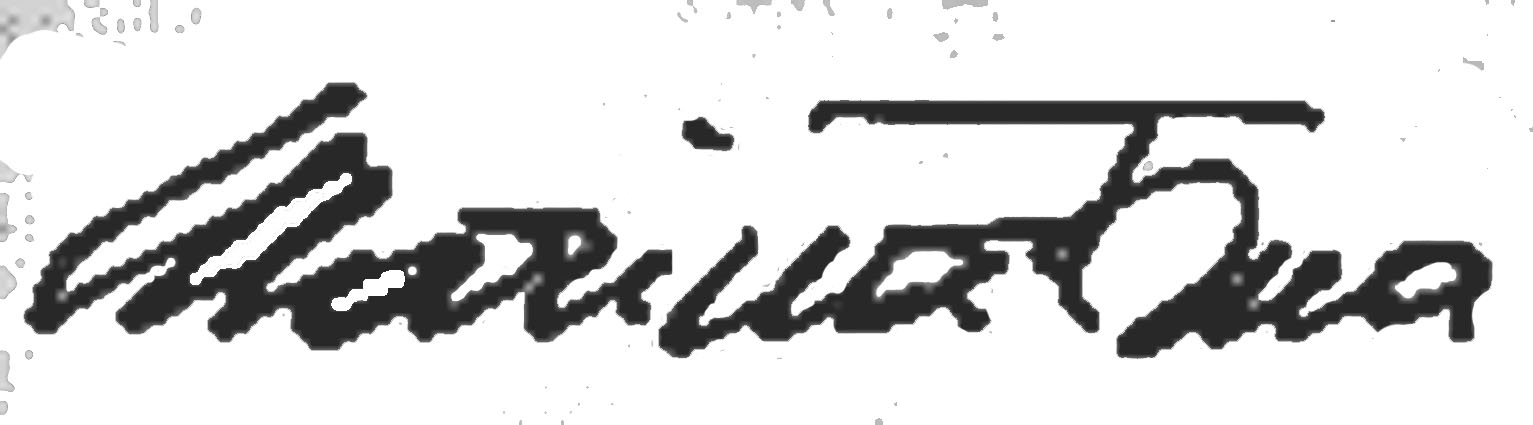
\includegraphics[width=\textwidth]{marina_frua_firma.jpg}
	\caption{}
	\label{fig:marina_frua_firma}
\end{figure}

\clearpage
